%\section{Motivation}

% Motivação: contextualização do problema ou da necessidade que motivou o trabalho. Essa seção deve preparar o leitor para a <Pergunta da Pesquisa>

According to the World Health Organisation (WHO), there are at least 2.2 billion people with some visual impairment degree \cite{world2019world}. Among them, 43,3 million are classified as blind and 295 million have moderate or severe vision impairment. In order to be fully integrated in our society, they rely on assistive devices, such as canes, braille speakers, among others \cite{bourne2021trends}. 

Although a range of products have already been proposed, incorporating different features, they do not completely fulfil their aim. Among the problems of the solutions available in the market are the lack of practicality and portability, being invasive and requiring too much effort to learn \cite{lozano2009electrotactile}.

The difficulty to use or learn how to use, a device could be avoided if concepts from human factors, or ergonomics, were analysed during the product’s development, using appropriate methods. The early application of these methods and tests could be a gamechanger for the success of the product's user experience \cite{wolf2019towards}.

Motivated by the dissatisfaction of blind people with the current available products, this dissertation starts from the hypothesis that a human-factors centred design of assistive devices for blind and visually impaired people (BVIs) requires the involvement of BVIs in the design process, in order to evaluate the product under design. The user has to experience the product under development in order to provide feedback to the design team on which to improve the product.

In order to approach this problem, this work proposes the use of Virtual Reality (VR) as a tool for creating virtual environments where proof of concepts or prototypes of assistive devices could be easily tested by BVIs. VR can be used to create specific, immersive and interactive situations that could help the user to learn and train \cite{farrell2018learning}, as well as the developers to create more user-friendly products.

In a virtual environment, as long as the BVI is wearing a locating system, he/she can navigate through the environment. Any information about the scenario where the person is, such as the position of devices and their distances to the person, is known and could be extracted from the virtual platform. As a consequence, before actually implementing a prototype of the assistive device, the designer can test different ways of translating this information into inputs, providing a flexible, safe and easy way to having it evaluated by different users.

%At the beginning of February 2022, about 400 million people had been diagnosed with COVID-19 around the world \cite{ourworldindata_cases}. Purposing to try to slow the rate at which the virus spread, WHO recommended strategies like wearing face masks, washing hands regularly, social distancing, avoiding touching surfaces and staying at home .

As a second motivation, this dissertation considers the COVID-19 pandemic scenario that dominated the world scene during the last two years. In order to try to slow the rate at which the virus spread, WHO recommended strategies such as wearing face masks, washing hands regularly, social distancing, and avoiding touching surfaces that have not been disinfected \cite{who_2020}. Particularly for BVI people, these recommendations bring additional difficulties as the touch is one of the senses they rely on to compensate for the visual impairment. %Social distance is also a challenge as they are not able to determine when another person is approaching the separation limits recommend by health agencies (ref??). 
The BVI depends on others to do their daily activities \cite{jondani2021strategies}. The development of solutions that are able to guide a BVI in an environment respecting social distance and other recommendations is also considered in this work.

\section{Objectives}
\label{sec:objetivos}

 % Objetivo geral: é a proposta, contribuição ou a entrega que endereça a solução da pergunta da pesquisa

 This dissertation proposes the use of virtual reality as a tool for evaluating proofs of concept of assistive devices for blind and visual impaired people from a human-factors perspective. The purpose is to provide a flexible and easily configured way of testing different concepts of assistive devices in order to support an agile and user-centred development.

 This goal is related to the following research questions, which are investigated in this work:

 \begin{itemize}
    \item Is it possible to evaluate and compare concepts of assistive device from a human factors’ perspective in a virtual environment? What are the main limitations of the use of a virtual reality environment? \label{itm:obj_first}
    \item Do non-BVI users, when deprived from their vision, evaluate assistive devices in a similar way as BVI users? \label{itm:obj_second}
\end{itemize}
 
 % Objetivos específicos: para a consecução do objetivo geral, foram identificados os seguintes objetivos específicos
 
 In order to investigate these research questions and achieve the proposed goal, the following specific objectives are defined:
 
 \begin{itemize}
     \item Select a scenario for testing assistive devices and develop it in a virtual environment; \label{itm:subobj_first}
     \item Develop three concepts of assistive devices that use different senses to provide input to the BVI; \label{itm:subobj_second}
     \item Propose a set of methods for BVI to evaluate assistive devices from human factors perspective; \label{itm:subobj_third}
     \item Design and execute an experiment to evaluate the concepts of assistive devices in the virtual environment using the proposed methods. \label{itm:subobj_forth}
 \end{itemize}
 
 %\section{Reason}
 
 % Justificativa: há na literatura, certamente, vários trabalhos que endereçam o mesmo problema que você está pesquisando. Justifique porque você quer – ainda assim – pesquisar esse tema, posicionando o seu trabalho em relação aos demais autores.
 
 %We are entering the 4.0 Industry, where humans work beside robots that scan images in 3D, \textit{drive} autonomous cars and can print parts to assembly almost anything in the universe

\section{Resources and methods} 

%Recursos e métodos: para cada um dos objetivos específicos, foram definidos os seguintes recursos e métodos (...). Você tem que justificar que os objetivos específicos são factíveis

This work adopts an experimental approach in order to evaluate the proposal of this dissertation and investigate the questions stated in Section \ref{sec:objetivos}. 
The work is organized in the following steps, illustrated in Figure \ref{fig:steps_work}:

\begin{enumerate}[label = Step \arabic* -- ]
    \item Literature review 
    
    It is composed of two parts. The first one is to review the fundamental concepts related to the topics covered in this work: human factors and virtual reality. The second part aims at contextualizing the dissertation’s proposal. It reviews recent published works on development and evaluation of assistive devices for BVI people.
    
    \item Specification of examples of virtual environment and assistive devices

    This step consists of specifying one example of virtual environment and a few examples of assistive device in order to test the proposed approach of using virtual reality for evaluating purposes. Considering the aforementioned motivation related to the covid-19 pandemic, the chosen virtual environment is the reception of a health clinic. The assistive devices used as examples are: audio system, haptic belt and virtual cane, which could be used as stand-alone devices or combined among them.
    
    \item Development of the specified virtual environment
    
    The virtual environment of a health clinic reception is developed in the Unit3D environment. The HTC VIVE VR Head Mounted Device (HMD) is used as localizing system to define the position of the user in the virtual environment.
    
    \item Development of proofs of concept of the specified assistive devices
    
    The three examples of devices are developed using the low cost and available equipment at the laboratory. The audio guide is developed using the audio system of HTV VIVE HMD, while the virtual cane is developed using the HTC VIVE VR hand controller. Finally, the haptic belt is develop using an ESP32 microcontroller, 8 vibrating motors 1027 and 3D printed pieces.
    
    \item Design and execution of the experiment
    
    The proposed experiment is based on the best practices and principles of Design of Experiment (DoE) discipline.
    The following techniques and tools are used for evaluating human factors:
    \begin{enumerate}[label = \alph*)]
        \item Questionnaires adapted from the literature, such as NASA-TLX and SAGAT, or proposed specifically for this work;
        \item Physiological sensors, such as GSR and ECG, to capture the body response.
    \end{enumerate}
    
    \item Analysis of results
    
    The results of the experiment are analysed graphically and statistically in order to estimate the user workload and situation awareness. In the statistical analysis, the outputs are verified for normality distribution, then pairwise compared using the Student’s T-Test, and their variance inside the group is verified using an ANOVA. Finally, when needed, a Fisher’s Least Squared Difference Test is done to verify similarities between pairs.

\end{enumerate}

\begin{figure}[!htb]
    \centering
    %\tikzstyle{every node}=[font=\large]

    \tikzstyle{start} = [rectangle, rounded corners, minimum width=3cm, minimum height=1.0cm,text centered, draw=black, fill=white!30, text width=3cm]
    \tikzstyle{steps} = [rectangle, minimum width=3cm, minimum height=1.0cm, text centered, draw=black, fill=white!30, text width=3cm]
    
    \tikzstyle{arrow} = [ccmDBlue, rounded corners, line width = 1mm, ->]
    
    \begin{tikzpicture}[node distance=2.5cm]
        \centering
        \node (start) [start] {Dissertation};

        \node (review) [steps, below of=start] {Literature Review};
        \draw [arrow] (start) to node[midway,right]{} (review);

        \node (examples) [steps, below of=review] {Examples specification};
        \draw [arrow] (review) to node[midway,right]{} (examples);
        
        \node (ve) [steps, below of=examples, left of = examples] {VE Development};
        \draw [arrow] (examples) to ++(0,-1.25cm) to ++(-2.5cm,0) to node[midway,right]{} (ve.north);
        
        \node (devices) [steps, below of=examples, right of = examples] {Devices development};
        \draw [arrow] (examples) to ++(0,-1.25cm) to ++(2.5cm,0) to node[midway,right]{} (devices.north);

        \node (experiment) [steps, below of=devices, left of = devices] {Experiment};
        \draw [arrow] (ve) to ++(0,-1.25cm) to ++(2.5cm,0) to node[midway,right]{} (experiment.north);
        \draw [arrow] (devices) to ++(0,-1.25cm) to ++(-2.5cm,0) to node[midway,right]{} (experiment.north);

        \node (analysis) [steps, below of=experiment] {Analysis of results};
        \draw [arrow] (experiment) to node[midway,right]{} (analysis);
    \end{tikzpicture}
        \centering
        \caption{Steps of this work}
        \label{fig:steps_work}
\end{figure}
\FloatBarrier

%\begin{itemize}
%    \item To answer about the feeling of presence from BVI users in VE:
%    \begin{itemize}
%        \item HTC VIVE VR Head Mounted Device (HMD), as show in Figure \ref{fig:htc_vive};
%        \item A guidance method evaluation questionnaires (See Appendix  \ref{sec:guidace_evaluation}) .
%    \end{itemize}
%    \item To answer if BVI users rely more on one type of information than the other and if non-BVI users can undergo the same situations as BVI users when using assistive products:
%    \begin{itemize}
%        \item Mental workload assessment, using:
%            \begin{itemize}
%                \item Physiological sensors (as show in Figure \ref{fig:sensores});
%                \item NASA-TLX questionnaire (See Appendix  \ref{sec:nasa_tlx}).
%            \end{itemize}
%            \item Situation awareness assessment, using:
%            \begin{itemize}
%                \item SAGAT questionnaire (Adapted for this experiment. See Appendix \ref{sec:sagat}).
%            \end{itemize}
%    \end{itemize}
%\end{itemize}
%
%\begin{figure}[!htb]
%    \begin{minipage}{.45\linewidth}
%        \centering
%        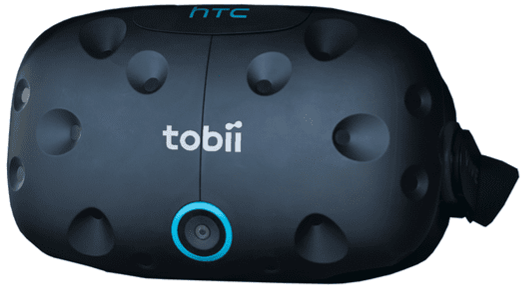
\includegraphics[width=\linewidth]{Introducao/VIVE.png}
%        \vspace{1.2cm}
%        \caption{VIVE HTC TOBII Virtual Reality Headset.}
%        \label{fig:htc_vive}
%    \end{minipage}
%    \begin{minipage}{.1\linewidth}
%        \hfill
%    \end{minipage}
%    \begin{minipage}{.45\linewidth}
%        \centering
%        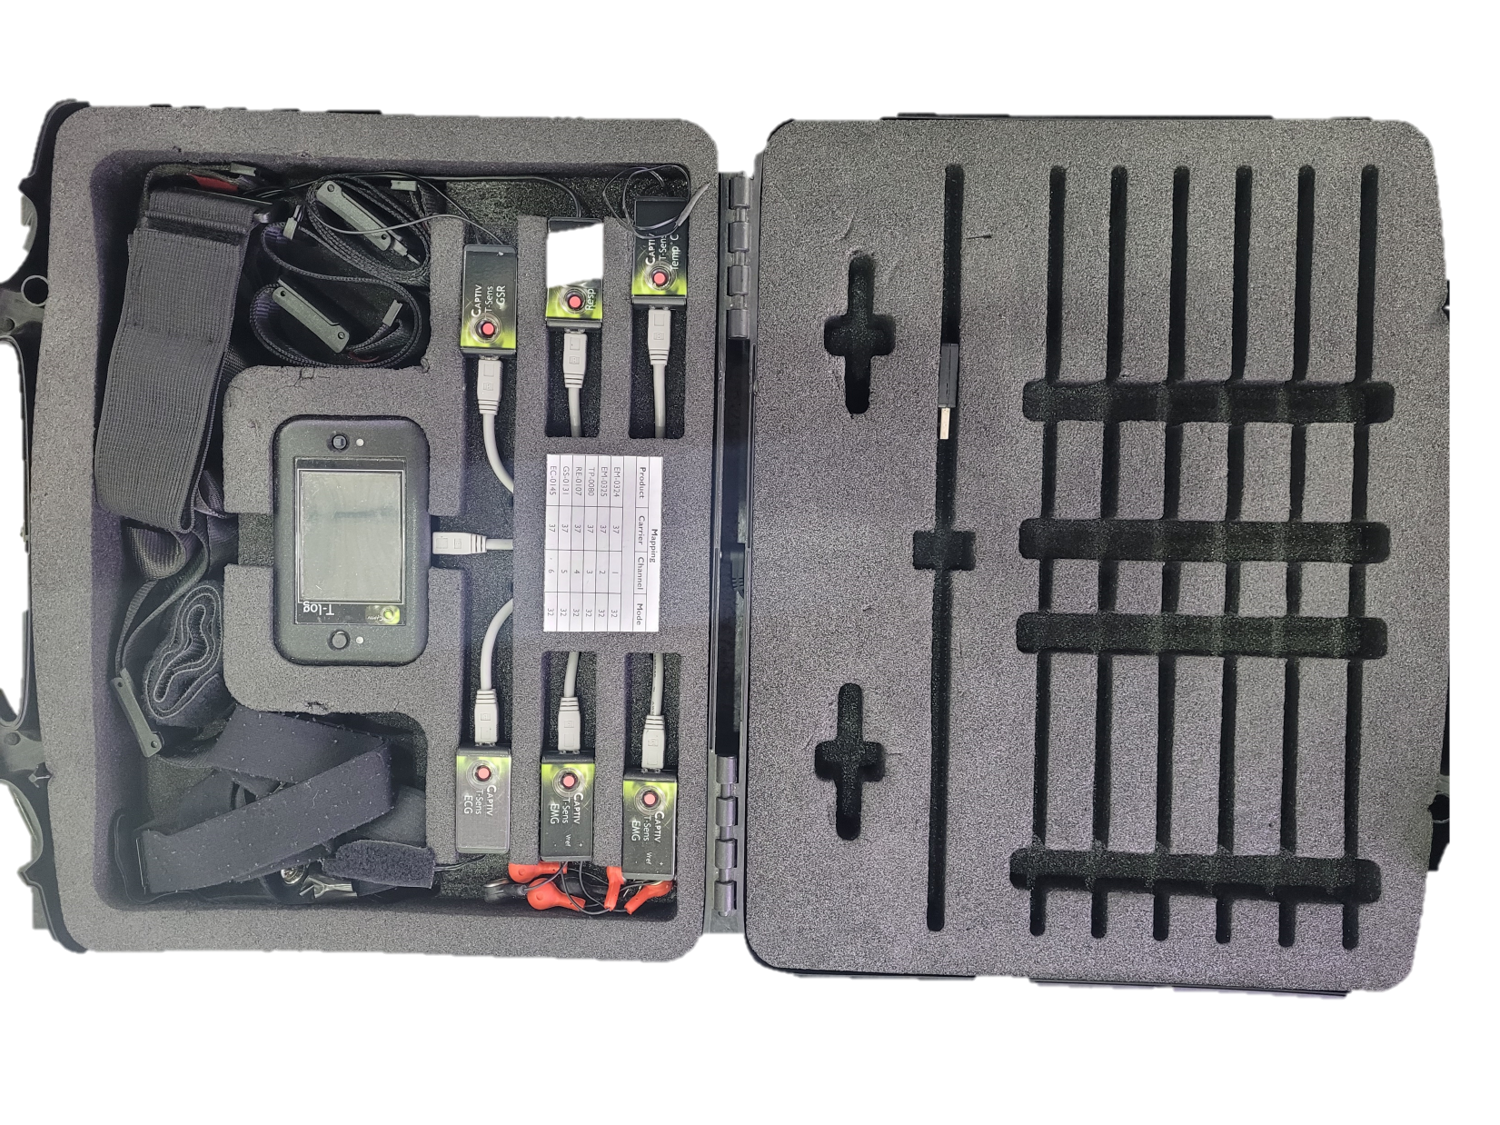
\includegraphics[width=\linewidth]{Introducao/sensores.png}
%        \caption{Captive T-Sens sensors.}
%        \label{fig:sensores}
%    \end{minipage}
%\end{figure}

\section{Research boundaries}

% Delimitação da pesquisa: é o recorte do seu trabalho

The concepts of assistive devices presented as part of this work are used only as examples for investigating the research questions presented in Section \ref{sec:objetivos}. The challenges related to their full development up to high Technology Readiness Levels (TRLs) are out of the scope of this work, as well as their feasibility as commercial products are out of the scope of this work.

% Estrutura do texto

\section{Structure of the text}

This dissertation is organized in seven additional chapters as follows.

Chapter \ref{ch:fundamentacao} introduce the concepts and techniques that are used in this work. It starts with a review on human factors, with emphasis on mental workload and situational awareness, and introduces some human factors’ evaluation tools and techniques. Then, it presents the definitions of Virtual Reality (VR) and Extended Reality (XR) and, to conclude, discusses the concept of co-design.

Chapter \ref{ch:revisao} is dedicated to the state of art. It brings a review of literature and discusses published research works that are related to this dissertation. It covers the proposal and evaluation of BVI devices with emphasis on the analysis of human factors or virtual reality.

Chapter \ref{ch:metodologia} details the proposal of this dissertation describing how virtual reality could be used to integrate BVI users into the design process of assistive design. It illustrates the proposed method by applying it to evaluate three different assistive devices (audio guide, virtual cane and haptic belt), as well as their mixed use, in the environment of a hospital reception. 

Chapter \ref{ch:resultados} describes the experiment designed to evaluate the dissertation’s proposal and analyses the results in order to investigate the research questions of Section \ref{sec:objetivos}

Finally, Chapter \ref{ch:conclusao} summarizes the main conclusions of this work and discusses future work.
